\section{敏感性分析}

为检验结论对关键参数的稳健性，本节在保持其他条件不变的基础上，逐子问题对主观设定和不确定参数逐一扫描，观察核心结论是否符合预期。各扫描档位与结果汇总于表 \ref{tab:sensitivity}，详细过程见对应章节。

\begin{table}[htbp]
\centering
\caption{关键参数敏感性汇总}
\label{tab:sensitivity}
\begin{tabular}{llcl}
\toprule
子问题 & 参数档位 & 核心结果 & 判定 \\
\midrule
问题一 & 极差目标 vs 方差目标 & 极差改善25.2\%，方差优18.4\% & 结论一致 \\
问题二 & 碳排放上限 350$\to$232.9 kt & 成本 $+7.9\%$，低于下界无可行解 & 权衡平缓 \\
问题二 & A/B 最低利用率 0\%$\to$15\% & 成本 $+2.4\%$，5\%--10\% 区间平缓 & 稳健 \\
问题三 & 消纳上限放开至可用量 & 购电趋零、成本趋下界，脱离现实 & 受限消纳结论稳健 \\
问题四 & 峰谷价差 $\times1.0\to\times2.0$ & 成本线性增长，约1074 M/倍 & 无策略突变 \\
问题四 & 新能源 $\pm20\%$ & 成本/碳排放近似对称 $\pm10\%$/$\pm9\%$ & 线性响应 \\
\bottomrule
\end{tabular}
\end{table}

\subsection{问题一 对两目标选择的敏感性}

极差最小化目标即Alpha、方差最小化目标即Beta，二者是公平性与时序平滑性的权衡。在相同数据时段与任务集合上交替执行两种目标，Alpha与Beta各有千秋，但调度均显著优于均匀分配基线，核心结论对目标选择不敏感。

\subsection{问题二 碳约束与最低利用率的灵敏度}

碳排放上限收紧至下界时，成本增幅在预期内（$+7.9\%$），碳-成本权衡呈平缓Pareto前沿。有力的证据是A/B最低利用率在5\%--10\%区间内几乎不增加成本，却能保障低负载时段的基础算力供给。模型在该参数维度上保持稳健，曲线见图 \ref{fig:minutil}。

\subsection{问题三 受限消纳上限的敏感性}

若放开消纳上限至新能源可用量，购电趋近于零、成本趋近理想下界，该情形理论成立但不可能实现。碳排放方面，$\varepsilon<1.00$在六区域全部无可行解，主解已逼近下限（$\varepsilon_{\min}$为A/B/C区0.993--0.994、D/E/F区0.957--0.969）。另一方面，受限消纳下的主解，结论稳健，结果形态由碳排放刚性主导。

\subsection{问题四 峰谷价差与新能源波动的灵敏度}

峰谷价差缩放时，成本线性增长而碳排放基本不变，印证碳排放主要由任务决定，与电价关系不大。新能源出力波动下，成本与碳排放均近似线性对称变化，储能与跨区调度有效吸收了不确定性。两参数扫描结果分别见图 \ref{fig:sub4-sens-price}、\ref{fig:sub4-sens-renew}。

\begin{figure}[htbp]
    \centering
    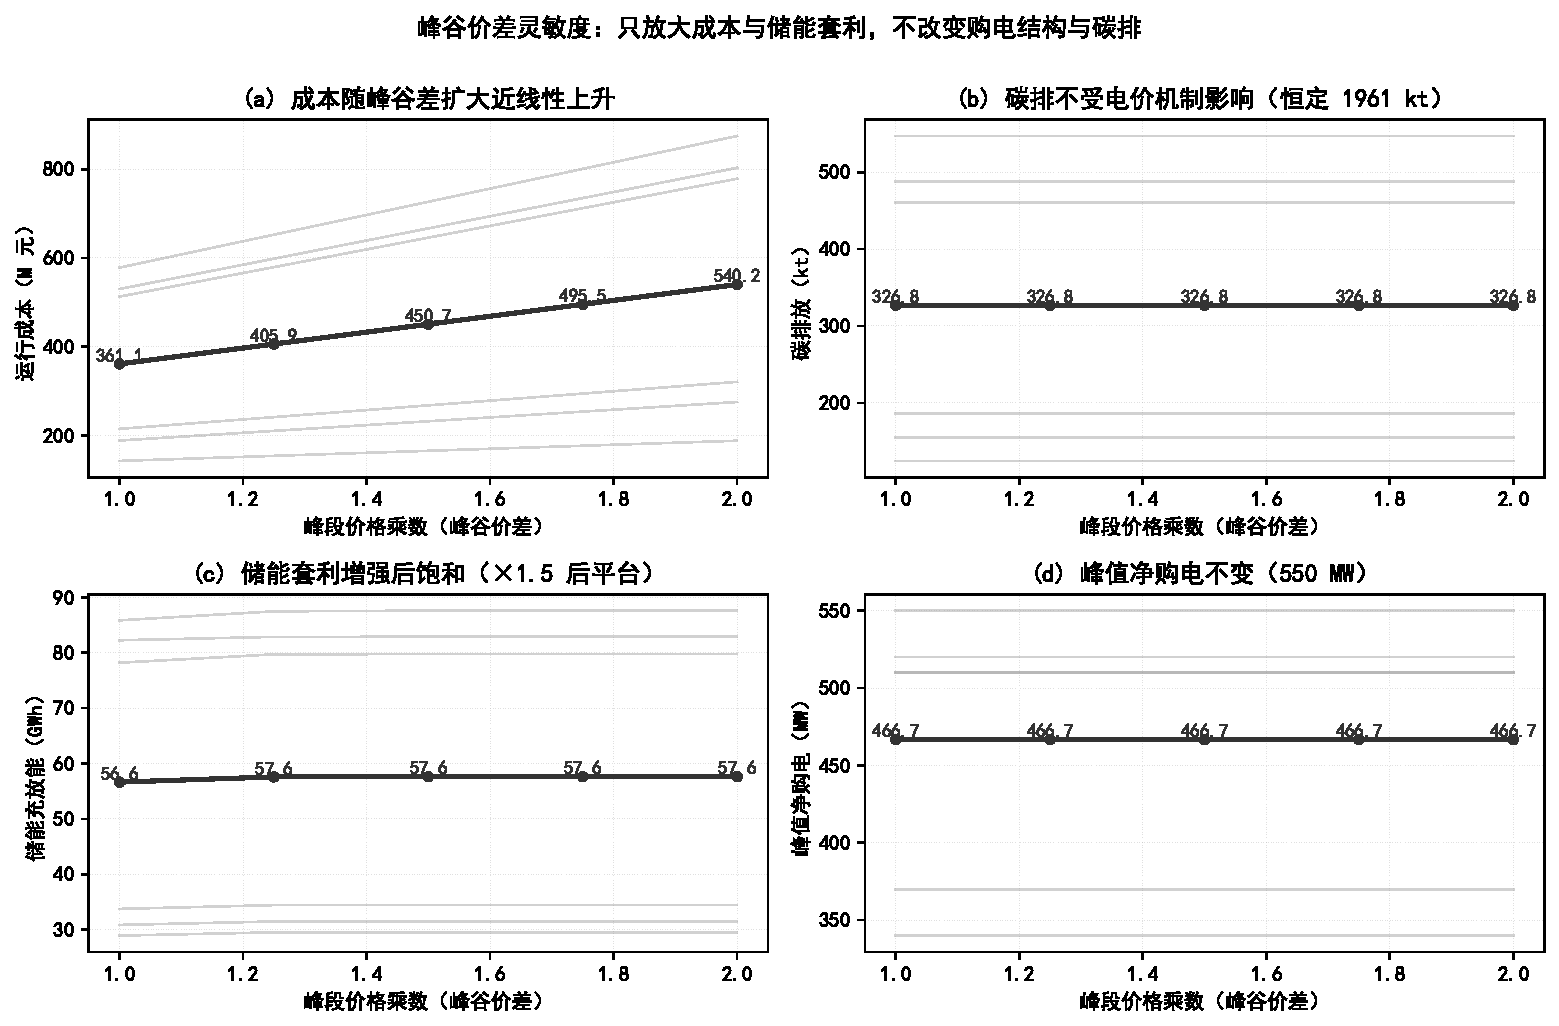
\includegraphics[width=0.8\textwidth]{../../outputs/figures/sub4-sens-price.pdf}
    \caption{峰谷价差缩放对成本与碳排放的影响（AI 辅助生成）}
    \label{fig:sub4-sens-price}
\end{figure}

\begin{figure}[htbp]
    \centering
    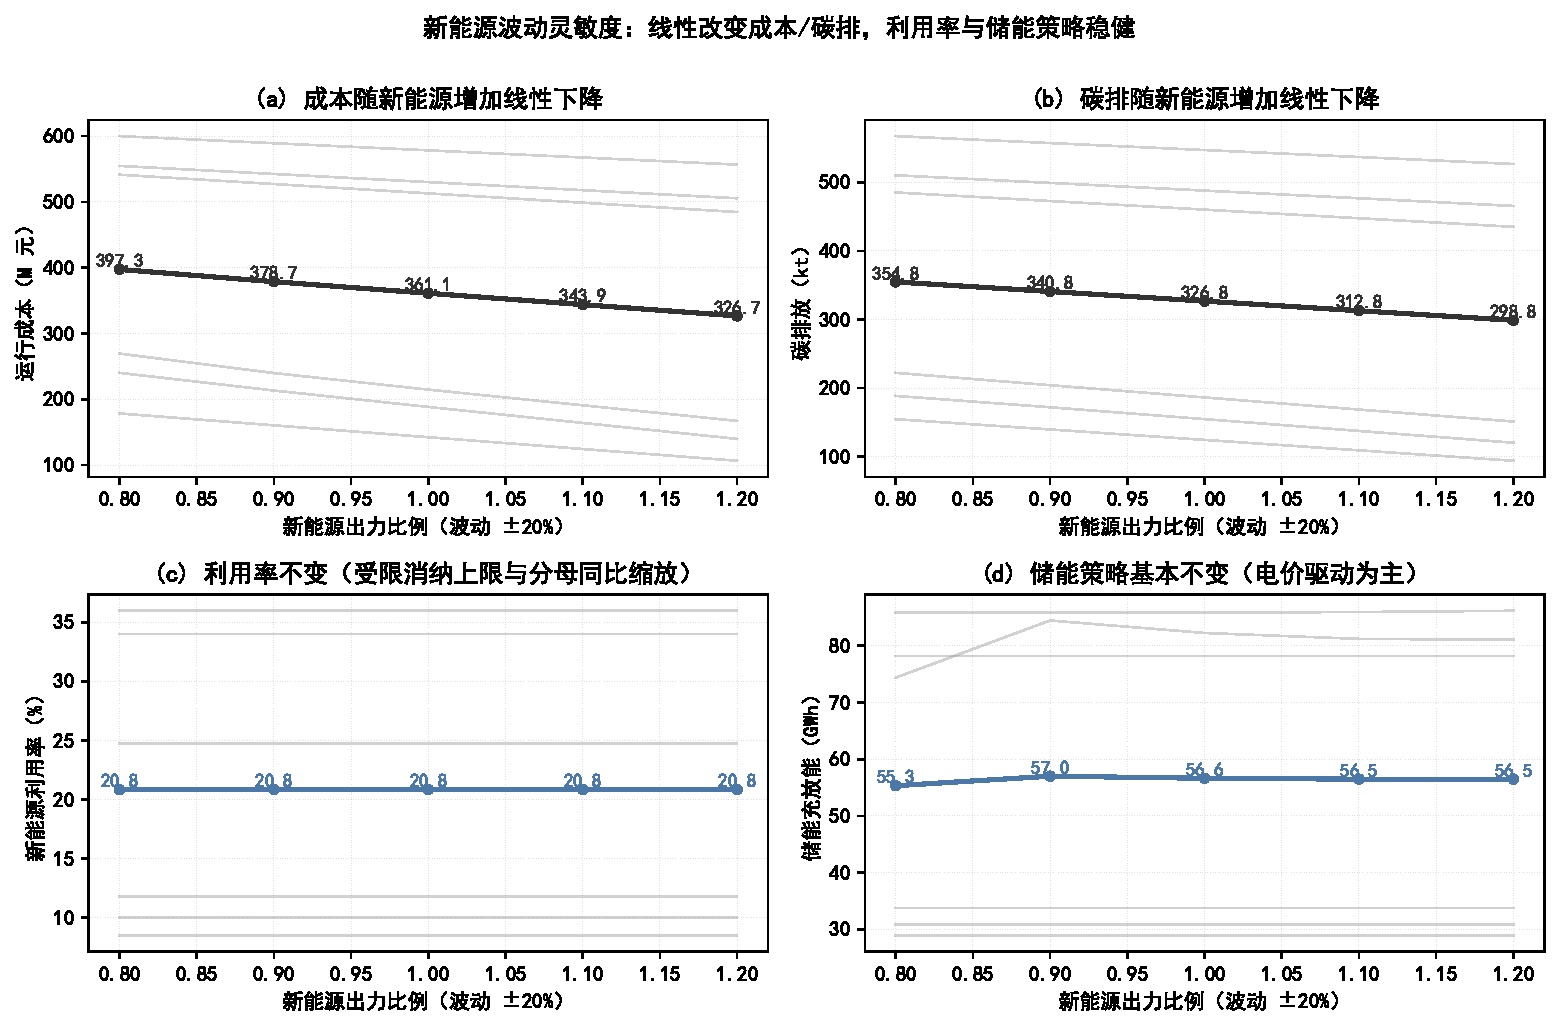
\includegraphics[width=0.8\textwidth]{../../outputs/figures/sub4-sens-renew.pdf}
    \caption{新能源 $\pm 20\%$ 波动对成本与碳排放的影响（AI 辅助生成）}
    \label{fig:sub4-sens-renew}
\end{figure}

\subsection{小结}

四个子问题的核心量化结论在参数扰动下方向正确、量级可控。极差与方差两种目标结论一致，碳约束收紧的成本增幅可控，碳排放已逼近可行域下界，峰谷价差与新能源波动均呈线性响应、无结构性翻转，模型整体稳健。
